\documentclass[UTF8]{ctexart}

\usepackage{graphicx, geometry, float}
\usepackage[most]{tcolorbox}
\geometry{left=2cm,right=2cm,top=2cm,bottom=2cm}

\tcbset{pikachu/.style={enhanced,colback=white,colframe=black,boxrule=0.6mm,enlarge top by=7.0mm,enlarge bottom by=2.0mm,top=50pt,sharp corners=south,arc=14mm,
overlay={
\begin{scope}[shift={([xshift=9.0mm,yshift=-13mm]frame.north west)},rotate=30]
% 左眼
  \path[draw=black,fill=black,line width=0.5mm] (0,0) arc (0:360:2mm);
  \path[fill=white] (-.05,.08) arc (0:360:1mm);
% 右眼
  \path[draw=black,fill=black,line width=0.5mm] (1.2,0) arc (0:360:2mm);
  \path[fill=white] (1.1-.05,.08) arc (0:360:1mm);
% 鼻子
  \path[draw=black,fill=black] (0.4,-.15) circle [x radius=0.06,y radius=0.03] (0:360);
% 嘴
  \path[draw=black,line width=0.4mm,xshift=0.5mm,yshift=-3.5mm] (0,-.02) .. controls (.1,-.1) and (.15,-.14) .. (.35,0) % 左
  .. controls (-.15+.7,-.14) and (-.1+.7,-.1) .. (0+.7,-.02); % 右
% 脸颊
  \path[draw=black,fill=white,line width=0.4mm] (1.6,-0.4) arc (10:290:2mm);
\end{scope}}
,
underlay={
\begin{scope}[shift={([xshift=0mm,yshift=0mm]frame.north west)}]
% 在耳朵和框架重叠的地方涂白(右)
  \path[draw=white,line width=0.7mm] (1.51,-0.03)--(2.55,-0.03);
% 在耳朵和框架重叠的地方涂白(左)
  \path[draw=white,line width=2.0mm] (0.1,-0.84)--(0.1,-2);
\end{scope}}
,
% 右耳
underlay={
\begin{scope}[shift={([xshift=0mm,yshift=0mm]frame.north west)}]
% 耳朵眼儿
  \path[draw=black,fill=white,line width=0.6mm,rounded corners=1.0pt] (1.5,-0.03) .. controls (2.5,0.3) and (3.5,-0.5) .. (3.7,-0.6) .. controls (2.7,-0.5) and (2.5,-0.5) .. (2.2,-0.4);

% 耳朵的黑色部分的边界
  \clip (1.5,-0.03) .. controls (2.5,0.3) and (3.5,-0.5) .. (3.7,-0.6) .. controls (2.7,-0.5) and (2.5,-0.5) .. (2.2,-0.4);

  \fill[black] (2.4,-0.5) to [out=10,in=210] (3.4,-0.3) -- (4,-0.7) -- cycle;
\end{scope}}
,
% 左耳
underlay={
\begin{scope}[shift={([xshift=9.06mm,yshift=4.93mm]frame.north west)},rotate=60]
% 耳朵向下反转
  \path[xscale=-1,draw=black,fill=white,line width=0.6mm,rounded corners=1.0pt] (1.5,-0.03) .. controls (2.5,0.3) and (3.5,-0.5) .. (3.7,-0.6) .. controls (2.7,-0.5) and (2.5,-0.5) .. (2.2,-0.4);

% 耳朵的黑色部分的边界
  \clip[xscale=-1] (1.5,-0.03) .. controls (2.5,0.3) and (3.5,-0.5) .. (3.7,-0.6) .. controls (2.7,-0.5) and (2.5,-0.5) .. (2.2,-0.4);

  \fill[xscale=-1,black] (2.4,-0.5) to [out=10,in=210] (3.4,-0.3) -- (4,-0.7) -- cycle;
\end{scope}}
,
% 尾巴
underlay={
\begin{scope}
[xscale=1.1,yscale=0.4,shift={([xshift=-5mm,yshift=-19mm]frame.north east)},rotate=38]
% [xscale=1,yscale=1,shift={([xshift=-8mm,yshift=-50mm]frame.north east)},rotate=0]
% 折线型尾巴1
% \draw [help lines] (-6,0) grid (6,6);
  \path[draw=black,fill=white,line width=0.6mm,rounded corners=1.0pt]
    (0,0) -- (0.3,0) -- (0.7,1.2) -- (-0.5,1.4) -- (-0.1,2.7) -- (-1.8,3) to [out=80,in=245] (-1,5.4) -- (-3.9,6) to [out=245,in=90] (-4.6,2.2) -- (-2,2) -- (-2.2,1.1) -- (0.2,0.7) -- cycle;

% 折线型尾巴2
  \clip (0,0) -- (0.3,0) -- (0.7,1.2) -- (-0.5,1.4) -- (-0.1,2.7) -- (-2,3) to [out=80,in=245] (-1.2,5.4) -- (-4.1,6) to [out=245,in=90] (-4.8,2.2) -- (-2.2,2) -- (-2.5,1.1) -- (0.2,0.7) -- cycle;
  \fill (-0.8,0.7) -- (-0.2,0.9) -- (-0.5,1.1) -- (-0.2,1.1) -- (-0.4,1.2) -- (-0.1,1.25) -- (-0.4,1.45)
    -- (1,1.5) -- (1,0) -- (-0.5,0) -- cycle;
\end{scope}}
,
% 后背上的花纹
underlay={
\begin{scope}[shift={(frame.north west)},rounded corners=10pt]
\path[fill=black,xshift=36mm,yshift=0mm] (0,0) -- (0.3,-0.8) -- (0.35,0);
\path[fill=black,xshift=42mm,yshift=0mm] (0,0) -- (0.3,-0.8) -- (0.35,0);
\end{scope}}
}}

\linespread{1.85}

\title{\vspace*{-2cm}双链表的设计与实现 实验报告}
\author{王笑同\quad 数学与应用数学(强基计划)2101\quad 3210105450}
\date{\today}

\begin{document}

\maketitle

\section{实验内容}

参考课本 91 页 3.5 节,在头文件 \verb|DoubleLinkedList.h| 中实现了双链表的所有基本操作,并在测试程序 \verb|main.cpp| 中实现了查找函数,这些操作包括:

\begin{tcolorbox}[pikachu]
    1. 获取链表中的节点个数,并判断链表是否为空;

    2. 清空链表;

    3. 获取链表头尾的节点值;

    4. 在链表的头尾插入新节点,并返回该新节点的迭代器;

    5. 在任意节点后插入新节点,并返回该新节点的迭代器;

    6. 删除链表头尾的节点;

    7. 删除链表中任意节点,并返回这一节点的下一节点的迭代器;

    8. 删除链表中一个区间内的所有节点,并返回这一区间右端点的下一节点的迭代器;

    9. 查找链表内首个值为指定值的节点,并返回其迭代器.
\end{tcolorbox}

其中涉及到返回节点迭代器的操作,若对应节点不存在,则返回指向空节点的迭代器.

\section{测试流程}

为了测试头文件 \verb|DoubleLinkedList.h|,我编写了测试代码 \verb|main.cpp|,其中实现了以下操作:

\begin{tcolorbox}[pikachu]
    1. 创建链表 \verb|l|;

    2. 用成员函数 \verb|push_back| 依次插入 $1,\,2,\,3,\,4,\,5$;

    3. 依次输出 \verb|l| 中的所有元素;

    4. 用 \verb|find| 函数查找链表中首个值为 $3$ 的节点;

    5. 删除链表中首个值为 $3$ 的节点;

    6. 再次输出链表 \verb|l| 中的所有元素.
\end{tcolorbox}

在 Ubuntu 下得到输出结果如下图:

\begin{figure}[H]
    \centering
    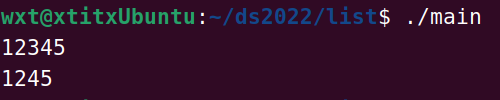
\includegraphics[scale=0.8]{figures/1.png}
    \caption{main.cpp 的运行结果}
\end{figure}

输出结果是符合预期的.

为了检测内存是否有泄露,使用 \verb|valgrind| 中的 \verb|memcheck| 工具:

\begin{figure}[H]
    \centering
    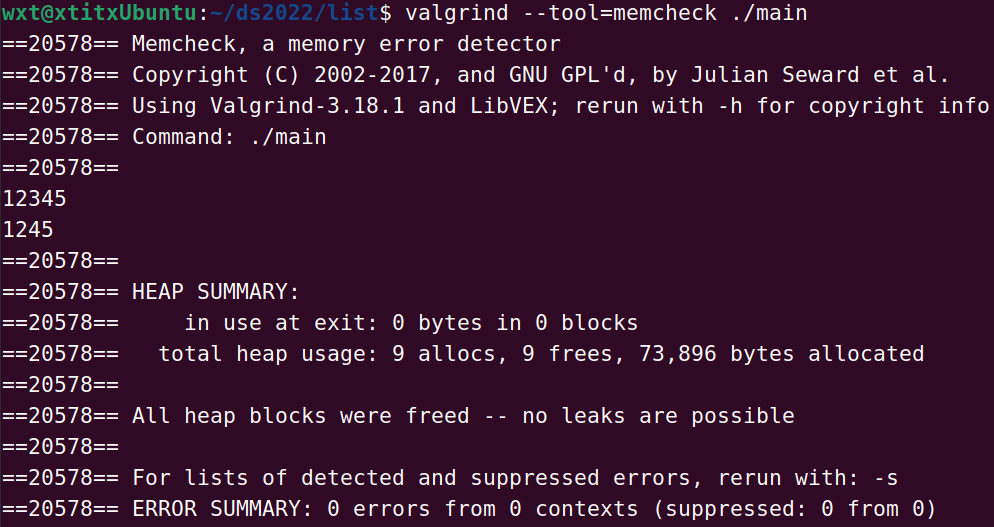
\includegraphics[scale=0.5]{figures/2.png}
    \caption{检测内存是否泄露}
\end{figure}

结果输出“No leaks are possible”,说明程序正常结束,无内存泄露可能.

\section{注记 \& 总结}

为了增强代码的可读性,我为两份代码都添加了必要的英文注释,且都采用 doxygen 格式,让代码更规范. 代码中也体现了一定的容错率,如 \verb|find| 函数中,即使没有找到符合要求的节点,程序也不会发生任何意外错误.

\end{document}